\documentclass[screen, aspectratio=169]{beamer}
\usepackage[T1]{fontenc}
\usepackage[utf8]{inputenc}

% Use the NTNU-temaet for beamer 
% \usetheme[style=ntnu|simple|vertical|horizontal, 
%     language=bm|nn|en, 
%     smalltitle, 
%     city=all|trondheim|alesund|gjovik]{ntnu2017}
\usetheme[style=ntnu, language=en, smalltitle]{ntnu2017}

\usepackage[english]{babel}
\usepackage[style=numeric,backend=biber,natbib=false,sorting=none]{biblatex}

\title[PCW-d1]{Physical Computing Workshop: Day 4}
\subtitle{Mini-Hackathon and the Real World}
\author[A. Xamb{\'o}]{Anna Xamb{\'o}}
\institute[NTNU]{Department of Music, NTNU}
\date{18 October 2019}
%\date{} % To have an empty date

\addbibresource{../pcw.bib} % Add bibliography database

% Set the reference style to numeric.
% See here: http://tex.stackexchange.com/questions/68080/beamer-bibliography-icon
\setbeamertemplate{bibliography item}[text] 

% Set bibliography fonts to a small size.
\renewcommand*{\bibfont}{\footnotesize}

\begin{document}

\begin{frame}
  \titlepage
\end{frame}
%
\usebackgroundtemplate{}
\begin{frame}
\frametitle{Warm-up Activity: Projects using Bela}
Pick one example of a project using Bela and explain it to the class in terms of input, behaviour and output. \\
You can find a number of examples on the Bela's blog: \url{https://blog.bela.io/}
\end{frame}
%
\begin{frame}
  \frametitle{Learning Outcomes}
  By the end of the session, you will be able to \dots
  \begin{itemize}
    \item Be able to express a concept from ideation to prototyping.
    \item Get a sense on how to combine and build on previous code.
    \item Explore how to design a custom-made musical instrument based on performance, engineering and originality/creativity.  
    \item Learn how to present a custom-made musical instrument.
    \item Demonstrate a custom-made musical instrument in a performance setting.
    \item Reflect on the custom-made musical instrument and performance using a blogging style.
  \end{itemize}
\end{frame}
%
\begin{frame}
  \frametitle{Overview of the Day}
      \begin{itemize}
	\item 9.15-9.45 Warm-up activity
	\item 9.45-10.00 Mini-hackathon explained
	\item 10.00-10.30 Ideation phase: definition of the concept to develop
	\item 10.30-11.00 Presentations of the concepts \& planning for the performance
	\item 11.00-14.30 Development of the prototype
	\item 14.30-15.00 Setting up
	\item 14.30-15.00 Final performance
	\begin{itemize}
	\item 15.00-15.10 Team A: Gaute, Rayam, Thibault and Ulrik
	\item 15.15-15.25 Team B: Jackson, Magda, Simon, and Jarle 
	\item 15.30-15.40 Team C: Aleksander, Paul, Tom Ignatius and Thomas
	\item 15.40-15.50 Popular vote of the best music hack
	\item 15.50-16.00 Award to the best team and closing
	\end{itemize}
    \end{itemize}  
\end{frame}
%
\usebackgroundtemplate{}
\begin{frame}
\frametitle{}
{\huge Mini-Hackathon}
\end{frame}
%
\begin{frame}
\frametitle{Theme}
{\Huge Recycle}
\end{frame}
%
\begin{frame}
  \frametitle{Ideation}
    \begin{itemize}
    	\item Meet for 30 minutes with your team and define the idea of your prototype. Some idea generation techniques include brainstorming, mindmapping, storyboarding, and so on. Here you can find some idea generation techniques: \url{https://www.cleverism.com/18-best-idea-generation-techniques/}
	\item For the presentation of the concept, you are only allowed to use 3 slides and you should bring a title of your prototype. Each group will have 10 minutes including Q\&A.
    \end{itemize}
\end{frame}
%
\begin{frame}
\frametitle{Performance}
\begin{itemize}
\item We should arrange the room during the morning: table on stage, seats for the audience: volunteers?
\item You will have 10 minutes to present the prototype and to perform. Try to pitch your idea and leave enough time to perform.  
\item Time will be strictly indicated (5 minutes, 2 minutes, 1 minute left). 
\item There are 5 minutes to setup, we will have a table on stage for each city.
	\begin{itemize}
	\item 15.00-15.10 Team A: Gaute, Rayam, Thibault and Ulrik {\scriptsize => Team C closeup camera Oslo/Trondheim}
	\item 15.15-15.25 Team B: Jackson, Magda, Simon, and Jarle  => {\scriptsize Team A closeup camera Oslo/Trondheim}
	\item 15.30-15.40 Team C: Aleksander, Paul, Tom Ignatius and Thomas => {\scriptsize Team B closeup camera Oslo/Trondheim}
	\item 15.40-15.50 Popular vote of the best music hack
	\item 15.50-16.00 Award to the best team and closing
	\end{itemize}
\item After the show, you will have to return your Bela kits in good condition.
\item After the show, we need volunteers on each city to reorganize the portal for Monday.
\end{itemize}	
\end{frame}
%
\begin{frame}
\frametitle{Pitch your Idea}
Some tips \& tricks on how to pitch a technology idea: ``18 Pitching Essentials: How to Pitch an Idea to Investors (and Early Customers)'': \url{https://www.ryrob.com/how-to-pitch/}
\end{frame}%
%
\begin{frame}
  \frametitle{Mini-hackathon \& Rehearsal}
  Each group has 3.5 hours to develop their idea and rehearse with the prototype and how they are going to pitch it. Try to be precise with the timing.
\end{frame}
%
\begin{frame}
  \frametitle{Post-activities}
    \begin{itemize}
         \item Fill in the post-questionnaire of the course.
    	\item Write a final blog post about the music hack (deadline: October 22, 2019 9.00). In the blog post, make sure to combine text with media to communicate the concept of your music hack, from ideation to the prototype. You will find guidelines on Canvas.
    \end{itemize}
\end{frame}
%
\begin{frame}
  \frametitle{Criteria of Evaluation (Audience)}
  The criteria of evaluation that will be promoted are the following:
    \begin{itemize}
    	\item Originality / Creativity
	\item Design / Engineering
	\item Performance / Musicality
    \end{itemize}
\end{frame}
%
\begin{frame}
  \frametitle{Prize}
  \begin{figure}
	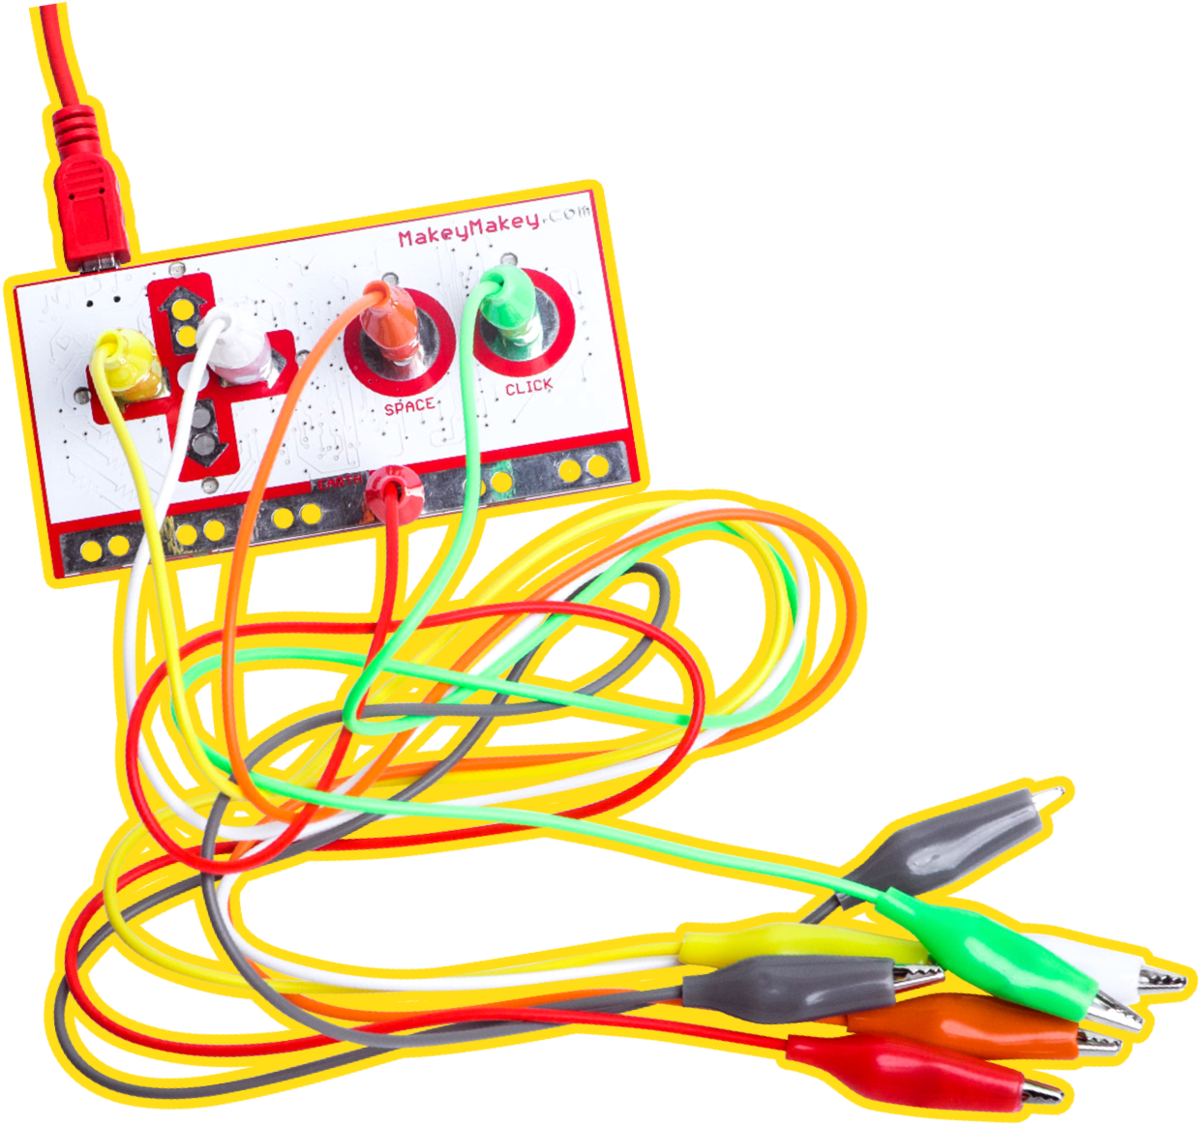
\includegraphics[scale=0.1]{img/makey-makey.png}
  \end{figure}
  The best music hack will be awarded with...
    \begin{itemize}
    	\item A \textbf{Makey Makey} kit for each team member!: \url{https://makeymakey.com/}
	\item Sponsored by Soundscape Studios.
    \end{itemize}
\end{frame}
%
\begin{frame}
  \frametitle{Happy Hacking!}
    \begin{figure}
	
\includegraphics[scale=0.3]{img/ethical-hacking.jpg}
    \end{figure}	
    {\tiny Image source: \url{https://www.indiatoday.in}}
\end{frame}
%

\end{document}
